%---------------------------------------------------------------------------------------------------------------%
\subsection{Esfera}
%---------------------------------------------------------------------------------------------------------------%
\subsubsection{Análise do Problema}
Para a construção da esfera teve-se que ter em conta coordenadas esféricas modificadas para o referencial rodado com Y para cima, Z como eixo das abcissas e X como eixo das ordenadas, como demonstra a Equação~\ref{eq:equ2}.


\begin{equation}
    \begin{cases}
    x = \cos(\phi) * \sin(\theta) * \rho \\
    y = \sin(\phi) * \rho \\
    z = \cos(\phi) * \cos((\theta) *\rho
    \end{cases}
\label{eq:equ2}
\end{equation}

Na Equação~\ref{eq:equ2}, $\rho$ representa o raio, $\phi$ o ângulo polar sendo $\phi \in [-\dfrac{\pi}{2}, \dfrac{\pi}{2}]$, $\theta$ representa o ângulo azimutal sendo $\theta \in [0, 2\pi]$. 


\newpage
\subsubsection{Diagrama}

\begin{center}
 	
 	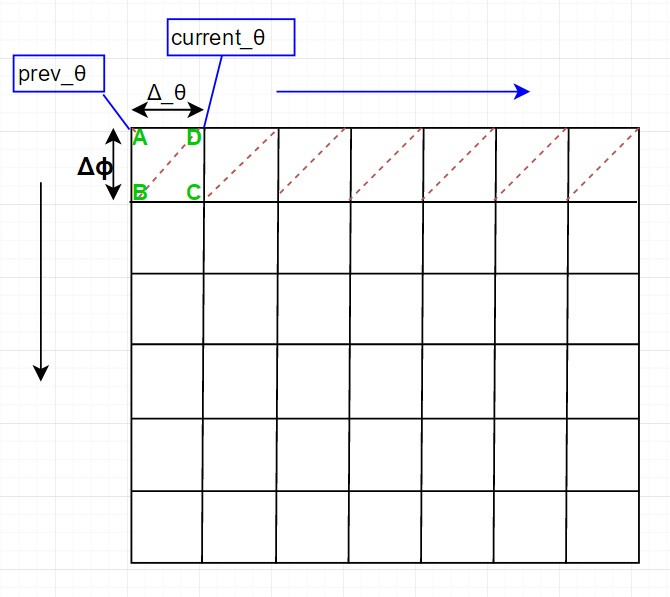
\includegraphics[width=\textwidth,height=\textheight,keepaspectratio]{resources/esferaw.jpg}
 	\captionsetup{type=figure, width=0.8\linewidth}
	\caption{Diagrama de representativo de construção de esfera}
\label{fig:ssec1:Digrama Esfera} 
\end{center}


No diagrama anterior pode-se ver uma matriz. A matriz representa a esfera nos graus de $\phi$ e $\theta$ para 6 \emph{stacks} e 7 \emph{slices}. Assim como um mapa representativo da Terra, pretende-se mostrar os pontos se a esfera fosse aplanada. 
Em cada quadrícula são calculados 4 pontos iniciais, com base nos cálculos apresentados pelo fórmula anterior. Note-se que, se usou duas variáveis para guardar o $\phi$ anterior e o $\phi$ corrente, e $\theta$ anterior  e $\theta$ corrente. Adicionalmente é calculada a diferença de graus entre \emph{slices} e \emph{stacks}, representados por $\delta \phi$ e $\delta \theta$, respetivamente. 

A intenção é calcular cada quadricula para cada linha e coluna, com auxilio das diferenças dos ângulos e à medida que se avança em cada quadricula, guardar o último grau calculado ($\phi$ e $\theta$) e calcular nos pontos com o incremento nestes ângulos. Assim desloca-se para a direita na matriz, conforme $\theta$ avança de 0 para $2\pi$ e para baixo, conforme $\phi$ avança de $\dfrac{\pi}{2}$ para $-\dfrac{\pi}{2}$ (sentido dos ponteiros do relógio).




\subsubsection{Figura}
\begin{center}
 	
 	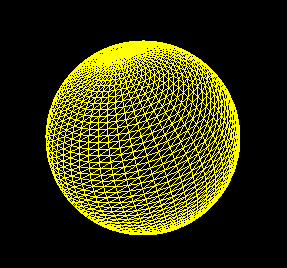
\includegraphics[width=\textwidth,height=\textheight,keepaspectratio]{resources/sphere.png}
 	\captionsetup{type=figure, width=0.8\linewidth}
	\caption{Esfera gerada}
\label{fig:ssec1:sphere} 
\end{center}
\newpage


\subsubsection{Algoritmo}

\begin{algorithm}
\floatname{algorithm}{Algoritmo}
\caption{Esfera}\label{euclid}
\begin{algorithmic}[1]
\State $\Delta\_\theta \gets \dfrac{2\pi}{slices}$

\State $\Delta\_\phi \gets \dfrac{2\pi}{stacks}$

\State $prev\_\phi \gets \dfrac{\pi}{2}$

\State $current\_\phi \gets prev\_\phi - \Delta\_\phi$





\State $i \gets 0$
\While{$i \leq stacks$} 
\State $prev\_\theta \gets 0$
\State $current\_\theta \gets \Delta\_\theta$

\State $j \gets 0$
\While{$j \leq slices$} 
\State $Ponto A \gets raio*\cos(prev\_\phi) * \sin(prev\_\theta),  
\newline raio*\sin(prev\_\phi),
\newline raio*\cos(prev\_\phi) * \cos(prev\_\theta)$

\State $Ponto B \gets raio*\cos(current\_\phi)*\sin(prev\_\theta),
\newline raio*\sin(current\_\phi),
\newline raio*\cos(current\_\phi) * \cos(prev\_\theta)$

\State $Ponto C \gets raio*\cos(prev\_\phi) * 
\newline \sin(current\_\theta),raio*\sin(prev\_\phi),
\newline raio*\cos(prev\_\phi) * \cos(current\_\theta)$

\State $Ponto D \gets raio*\cos(current\_\phi) *
\newline \sin(current\_\theta),raio*\sin(current\_\phi),raio*\cos(current\_\phi) * \newline \cos(current\_\theta)$

\State $i \gets j + 1$ 

\State $Triangulo(Ponto A, Ponto B, Ponto D)$

\State $Triangulo(Ponto B, Ponto C, Ponto D)$

\State $prev\_\theta \gets Current\_\theta$
\State $current\_\theta \gets Current\_\theta + \Delta\_\theta $
\EndWhile

\State $prev\_\phi \gets Current\_\phi$
\State $current\_\phi \gets Current\_\phi - \Delta\_\phi $
\State $i \gets i + 1$ 

\EndWhile

\end{algorithmic}
\end{algorithm}
